\section{Infimum, Supremum and Lattices}
\label{tree:poset:lattices}

We will now introduce the notion of infimum and supremum. The infimum of a
subset \(\S\) of a poset \(\P\) is an element \(l\) of \(\P\) satisfying the two
following conditions: \(l\) is a lower bound of \(\S\), meaning that \(l \le
s\) for all \(s \in \S\), and \(l\) is the largest such lower bound. From this
definition, it is easy to deduce the definition of the supremum of a subset
\(\S\) of a poset \(\P\).

From these two new terms we can now build the definition of a lattice. A
lattice is a poset \(\P\) in which any subset \(\S\) that is a pair of two
elements of \(\P\) has a unique infimum and a unique supremum. In lattice
theory, infima and suprema are sometimes called greatest lower bounds and least
upper bounds respectively.

An example of a lattice is the set of natural numbers (including zero)
partially ordered by divisibility. In this example, the infimum and the
supremum of a pair of elements are the greatest common divisor and the least
common multiple respectively. \ref{fig:poset:lattice:60div} illustrates this
example with the integer divisors of \(60\).

\begin{figure}
\center
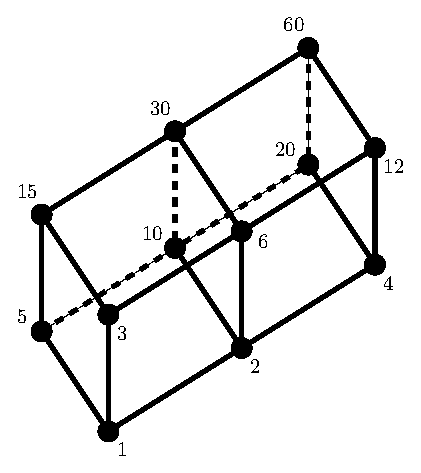
\includegraphics[height=0.2\textheight]{fig/poset/lattice/60div}
\caption{Hasse diagram of the set of integer divisors of \(60\) partially ordered by
divisibility.}\label{fig:poset:lattice:60div}
\end{figure}
